\documentclass{beamer}
\usetheme{Warsaw}

\usepackage{amsfonts}
\usepackage{amssymb}
\usepackage{amsbsy}
\usepackage{amsmath}
\usepackage{array}
\usepackage{xmpmulti}
\usepackage{textpos}

%\addtobeamertemplate{footnote}{}{\vspace{2ex}}
\setlength{\extrarowheight}{0.2cm}
\setlength{\arraycolsep}{0.08cm}

%\newtheorem{theorem}{Theorem}[section]
%\newtheorem{lemma}[theorem]{Lemma}
%\newtheorem{proposition}[theorem]{Proposition}
%\newtheorem{corollary}[theorem]{Corollary}

%\newenvironment{proof}[1][Proof]{\begin{trivlist}
%\item[\hskip \labelsep {\bfseries #1}]}{\end{trivlist}}
%\newenvironment{definition}[1][Definition]{\begin{trivlist}
%\item[\hskip \labelsep {\bfseries #1}]}{\end{trivlist}}
%\newenvironment{example}[1][Example]{\begin{trivlist}
%\item[\hskip \labelsep {\bfseries #1}]}{\end{trivlist}}
%\newenvironment{remark}[1][Remark]{\begin{trivlist}
%\item[\hskip \labelsep {\bfseries #1}]}{\end{trivlist}}

\renewcommand{\a}{\alpha}						
\renewcommand{\b}{\beta}
\renewcommand{\d}{\delta}						
\newcommand{\e}{\epsilon}
\newcommand{\g}{\gamma}
\newcommand{\h}{\eta}					
\renewcommand{\j}{\varphi}
\renewcommand{\l}{\lambda}					
\newcommand{\m}{\mu}
\newcommand{\n}{\nu}
\newcommand{\p}{\pi}
\renewcommand{\r}{\rho}
\newcommand{\s}{\sigma}							
\newcommand{\q}{\theta}
\renewcommand{\t}{\tau}								
\newcommand{\w}{\omega}
\newcommand{\y}{\psi}
\newcommand{\z}{\zeta}
\newcommand{\D}{\Delta}
\newcommand{\G}{\Gamma}
\renewcommand{\L}{\Lambda}
\newcommand{\Q}{\Theta}
\renewcommand{\S}{\Sigma}
\newcommand{\W}{\Omega}
\newcommand{\bgtilde}[1]{\tilde{\bg#1}}					%overset tilde bolded little greek letter
\newcommand{\bghat}[1]{\hat{\bg#1}}						%overset hat bolded little greek letter
\newcommand{\btilde}[1]{\tilde{\bm#1}}					%overset tilde on bolded letter
\newcommand{\bhat}[1]{\hat{\bm#1}}						%overset hat on bolded letter
\newcommand{\bi}{\begin{itemize}} 						%start bullet points
\newcommand{\ei}{\end{itemize}} 						%end bullet points
\newcommand{\bn}{\begin{enumerate}}						%start numbering
\newcommand{\en}{\end{enumerate}}						%end numbering
\newcommand{\bne}{\begin{equation}}						%begin numbered equation
\newcommand{\ene}{\end{equation}}						%end numbered equation
\renewcommand{\bf}{\textbf}								%bold font in text
\newcommand{\bm}{\mathbf}								%bold font in maths
\newcommand{\bg}{\boldsymbol}							%bold font in maths for small greek letters
\newcommand{\tf}{\textrm}								%text font in maths
\newcommand{\Def}[1]{\bf{Definition (#1):}}				%generic "definition" macro
\renewcommand{\i}{\item}								%item in bullet or numbered list
\newcommand\independent{\protect\mathpalette{\protect\independenT}{\perp}}	%independence symbol
\def\independenT#1#2{\mathrel{\rlap{$#1#2$}\mkern2mu{#1#2}}}				%independence symbol (cont'd)
\newcommand{\cov}{\textrm{cov}}							%covariance
\newcommand{\Acov}{\textrm{Acov}}						%aymptotic covariance
\renewcommand{\skew}{\textrm{skew}}						%skewness
\newcommand{\kurt}{\textrm{kurt}}						%kurtosis
\newcommand{\plim}{\textrm{plim}}						%probability limit
\newcommand{\as}{\textrm{a.s.}}							%almost surely
\newcommand{\ms}{\textrm{m.s.}}							%mean square
\newcommand{\ra}{\rightarrow}
\newcommand{\ConT}{\overset{T \rightarrow \infty}{\xrightarrow{\hspace*{0.75cm}}}} %converges T goes to infinity
\newcommand{\ConN}{\overset{N \rightarrow \infty}{\xrightarrow{\hspace*{0.75cm}}}} %converges N goes to infinity
\newcommand{\ConP}{\overset{\P}{\longrightarrow}}		%converges in probability
\newcommand{\ConAS}{\overset{\as}{\longrightarrow}}		%converges almost surely
\newcommand{\ConMS}{\overset{\ms}{\longrightarrow}}		%converges in mean square
\newcommand{\ConD}{\overset{\tf{d}}{\longrightarrow}}	%converges in distribution
\newcommand{\ConLOne}{\overset{\mathcal{L}_1}{\longrightarrow}}		%converges in L1
\newcommand{\ConLTwo}{\overset{\mathcal{L}_2}{\longrightarrow}}	%converges in L1
\newcommand{\ADis}{\overset{\tf{a}}{\backsim}}			%asymptotically distributed as
\newcommand{\N}{\mathcal{N}}							%normal distribution "N"
\newcommand{\snormal}{\N(0,1)}							%standard normal
\newcommand{\unormal}{\N(\m,\s^2)}						%univariate normal
\newcommand{\vnormal}{\N(\bg{\m},\bm{\S})}				%vector normal
\newcommand{\vsnormal}{\N(\bm{0},\bm{I})}				%vector standard normal
\newcommand{\ulnormal}{\tf{Log-}\N(\m,\s^2)}			%univariate log-normal
\newcommand{\norm}[1]{\left|\left|#1\right|\right|}		%norm
\newcommand{\abs}[1]{\left|#1\right|}				 	%absolute value
\newcommand{\tran}{\mathsf{T}}							%transpose
\newcommand{\tr}{\mathrm{tr}}							%trace
\newcommand{\adj}{\mathrm{adj}}							%adjoint (of a matrix)
\newcommand{\sumtT}{\sum_{t=1}^T}						%sum from t=1 to T
\newcommand{\sumnN}{\sum_{n=1}^N}						%sum from n=1 to N
\newcommand{\sumkK}{\sum_{k=1}^K}						%sum from k=1 to K
\renewcommand{\P}{\mathbb{P}}							%blackboard style "P" for probability
\newcommand{\E}{\mathbb{E}}								%blackboard style "E" for expecatation
\newcommand{\V}{\mathbb{V}}								%blackboard style "V" for variance
\newcommand{\R}{\mathbb{R}}								%blackboard style "R" to denote real number line
\newcommand{\CalF}{\mathcal{F}}							%mathcal style "F" to denote filtration
\newcommand{\CalG}{\mathcal{G}}							%mathcal style "G" to denote a grid
\newcommand{\CalH}{\mathcal{H}}							%mathcal style "H" to denote a sub-grid
\newcommand{\CalA}{\mathcal{A}}							%mathcal style "A" to denote some set
\newcommand{\CalB}{\mathcal{B}}							%mathcal style "B" to denote some set
\newcommand{\blue}[1]{{\color{blue}#1}}					%colour the text blue
\newcommand{\red}[1]{{\color{red}#1}}					%colour the text red
\newcommand{\green}[1]{{\color{green}#1}}					%colour the text red
\newcommand{\yellow}[1]{{\color{yellow}#1}}					%colour the text red
\newcommand{\can}{\citeasnoun}							%Used as a shortcut for the citation command


%----------------------------------- CUSTOM COMMANDS ---------------------------------------------------%
\newcommand{\qh}{\hat{\theta}}
%\newcommand{\qt}{\tilde{\theta}}
\newcommand{\qt}{y}
\newcommand{\qtt}{\tilde{\tilde{\theta}}}
\newcommand{\db}{\bar{d}}


\def\newblock{\hskip .11em plus .33em minus .07em}
\title[{\makebox[.45\paperwidth]{\hfill \insertframenumber/\inserttotalframenumber}}]{Robust Statistics and Financial Data}  
\author{Colin T. Bowers}
\institute{Macquarie University, \newline colintbowers@gmail.com, \newline https://github.com/colintbowers/RobustStatsTutorial.jl}
\date{2016-09-14}
\begin{document}		

\begin{frame}	

\maketitle

\end{frame}

\setbeamercovered{dynamic}
\setbeamertemplate{bibliography item}{}
%\setbeameroption{show notes} %un-comment to see the notes
%\setbeamertemplate{note page}[plain] %un-comment to print plain version of notes


%\section{Introduction}
%
%\begin{frame}
%\frametitle{Preview}
%\begin{center}
%\LARGE{Section 1: The peculiar phenomenon}
%\end{center}
%\end{frame}





	
\section{Basic Intuition}

\begin{frame}
\frametitle{Preview}
\begin{enumerate}
\item Basic intuition and the trimmed mean
\item Measuring tail fatness
\item Fat tails in financial returns
\item The trimmed mean and financial returns
\item Robust estimation of a linear model for financial returns
\item Traps and pitfalls when using robust statistics
\end{enumerate}
\end{frame}





\begin{frame}
\frametitle{Fat-tailed data}
\begin{center}
\begin{picture}(200,100) \put(-60,-20){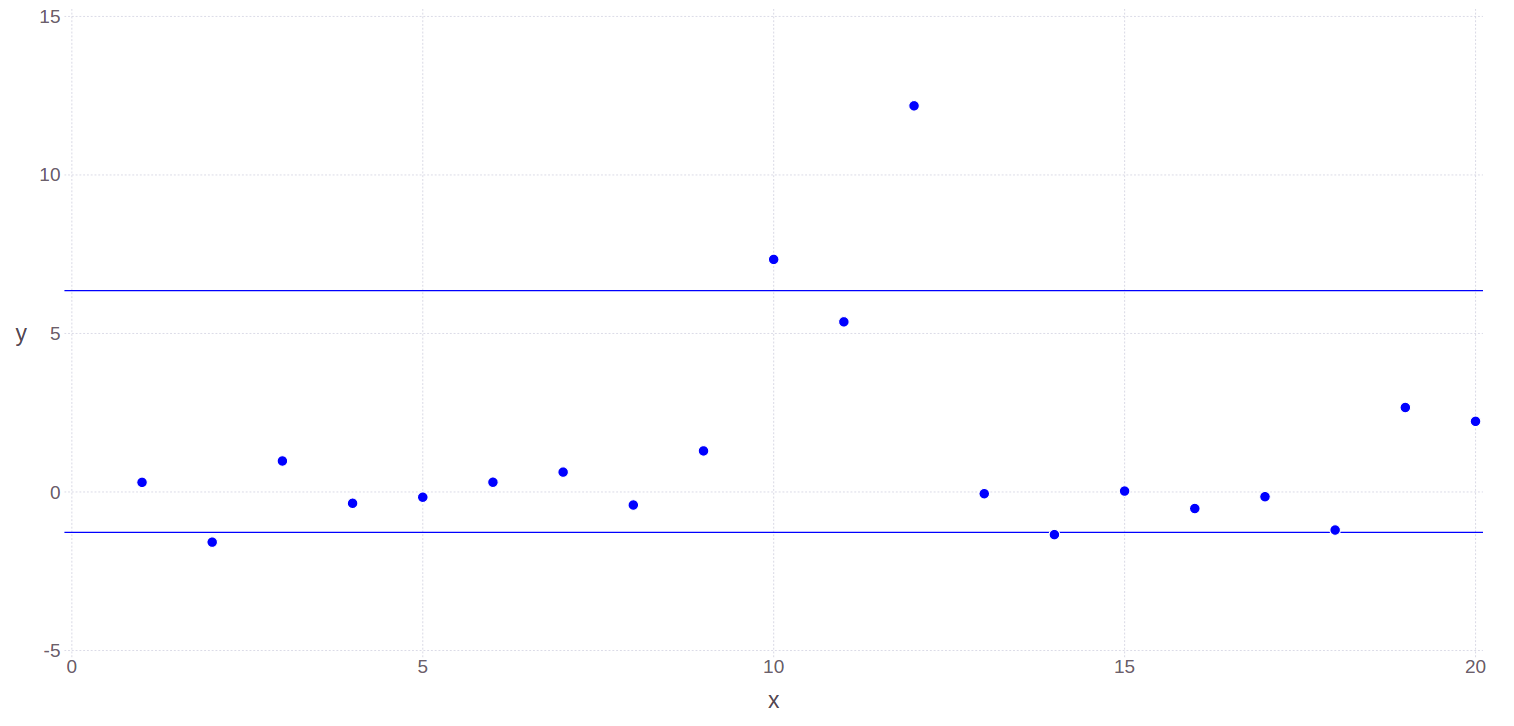
\includegraphics[height=4.5cm]{tDistDataCutoff}} \end{picture}
\end{center}
\vspace{0.3cm}

20 observations from the Student-t (2 DoF*) Distribution
\begin{itemize}
\item True mean  = 0
\item Sample mean = 1.38
\item Trimmed mean = 0.68
\end{itemize}
\scriptsize{*DoF = Degrees of Freedom}
\end{frame}



\begin{frame}
\frametitle{The trimmed mean}
\begin{center}
\begin{picture}(200,100) \put(-60,-30){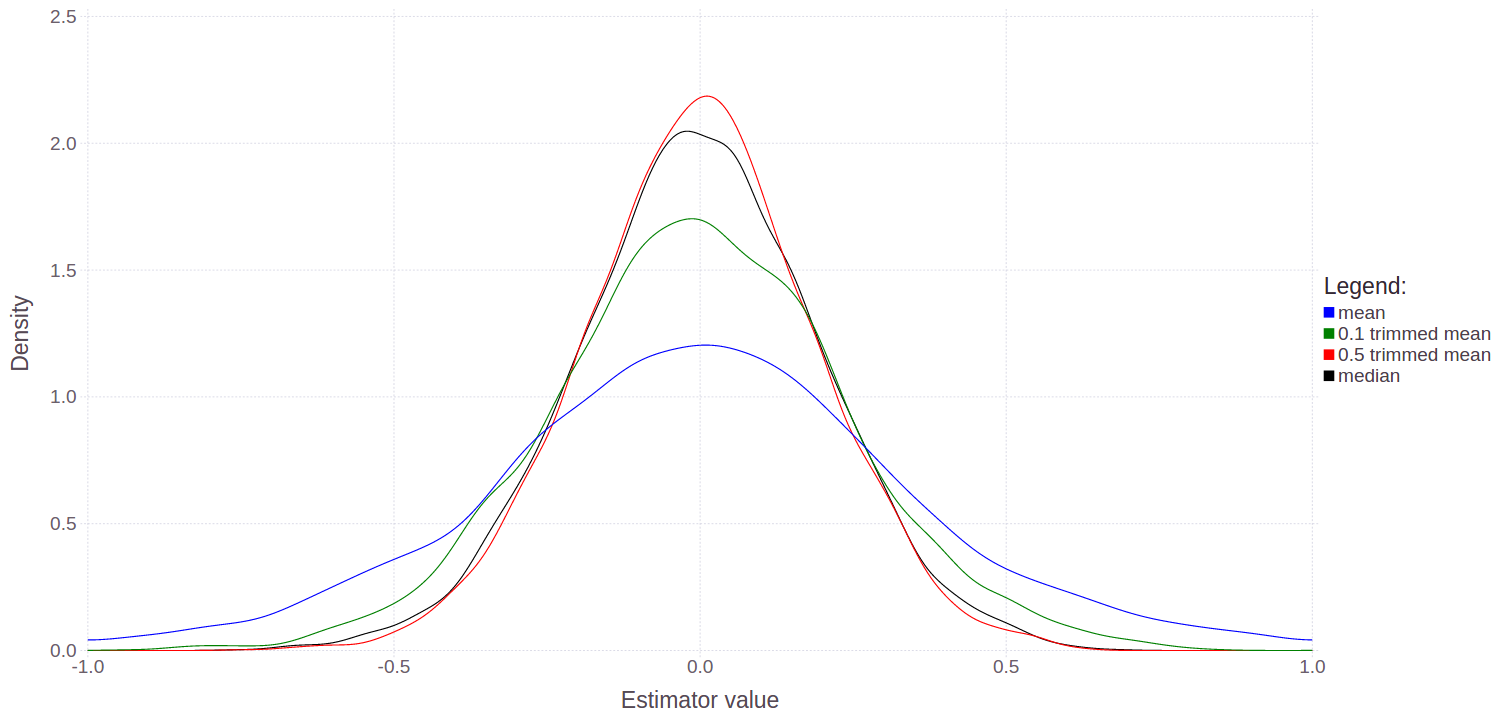
\includegraphics[height=5.0cm]{tDistDataEstDensity}} \end{picture}
\end{center}
\vspace{0.75cm}
Simulated kernel density estimate for the trimmed mean given a Student-t (2 DoF) DGP*

\scriptsize{*DGP = Data Generating Process}
\end{frame}



\section{Tail Fatness}



\begin{frame}
\frametitle{Measures of tail fatness}
Standard textbook definition:
\begin{equation}
Kurtosis = \frac{\E(X - \m)^4}{(\V X)^2}
\end{equation}
\red{Problem}: What if $\E X^4 \ra \infty$?
\vspace{0.5cm}

\blue{Solution}: Hogg's robust kurtosis:
\begin{equation}
Robust Kurtosis = \frac{\E (X \mathbb{I}\{X > Q_{0.95}\}) - \E (X \mathbb{I}\{X < Q_{0.05}\})}{\E (X \mathbb{I}\{X > Q_{0.5}\}) - \E (X \mathbb{I}\{X < Q_{0.5}\})}
\end{equation}
where $Q_p$ is the quantile associated with probability $p$.

%\blue{Solution}: Hogg's robust kurtosis. Let $I(a, b) = \int_a^b x dF(x)$ where $F(x)$ is the cdf of $X$. Then:
%\begin{equation}
%Robust Kurtosis = \frac{I(Q_{0.95}, Q_{\infty}) - I(Q_{-\infty}, Q_{0.05})}{I(Q_{0.5}, Q_{\infty}) - I(Q_{-\infty}, Q_{0.5})} ,
%\end{equation}
%where $Q_p$ is the quantile associated with probability $p$.
\end{frame}


\begin{frame}
\frametitle{Hogg's robust kurtosis numerator}
Numerator: $\E (X \mathbb{I}\{X > Q_{0.95}\}) - \E (X \mathbb{I}\{X < Q_{0.05}\})$
\begin{center}
\begin{picture}(200,100) \put(-30,-40){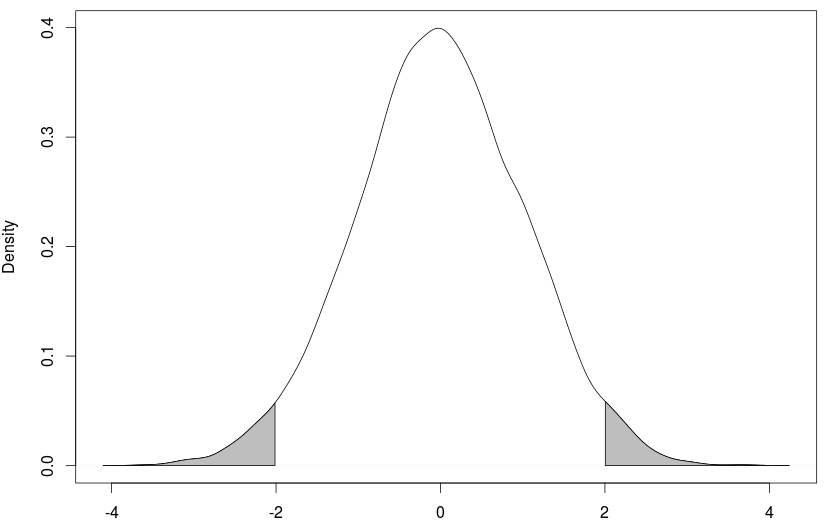
\includegraphics[height=5.0cm]{TailsShaded5Percent}} \end{picture}
\end{center}
\end{frame}



\begin{frame}
\frametitle{Hogg's robust kurtosis denominator}
Denominator: $\E (X \mathbb{I}\{X > Q_{0.5}\}) - \E (X \mathbb{I}\{X < Q_{0.5}\})$
\begin{center}
\begin{picture}(200,100) \put(-30,-40){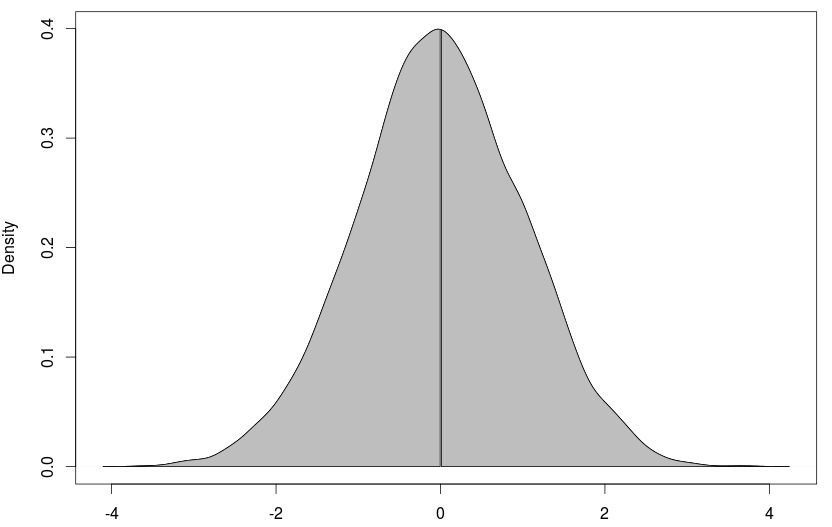
\includegraphics[height=5.0cm]{TailsShaded50Percent}} \end{picture}
\end{center}
\end{frame}



\begin{frame}
\frametitle{The problem with undefined moments}
\begin{center}
\begin{picture}(200,100) \put(-60,-30){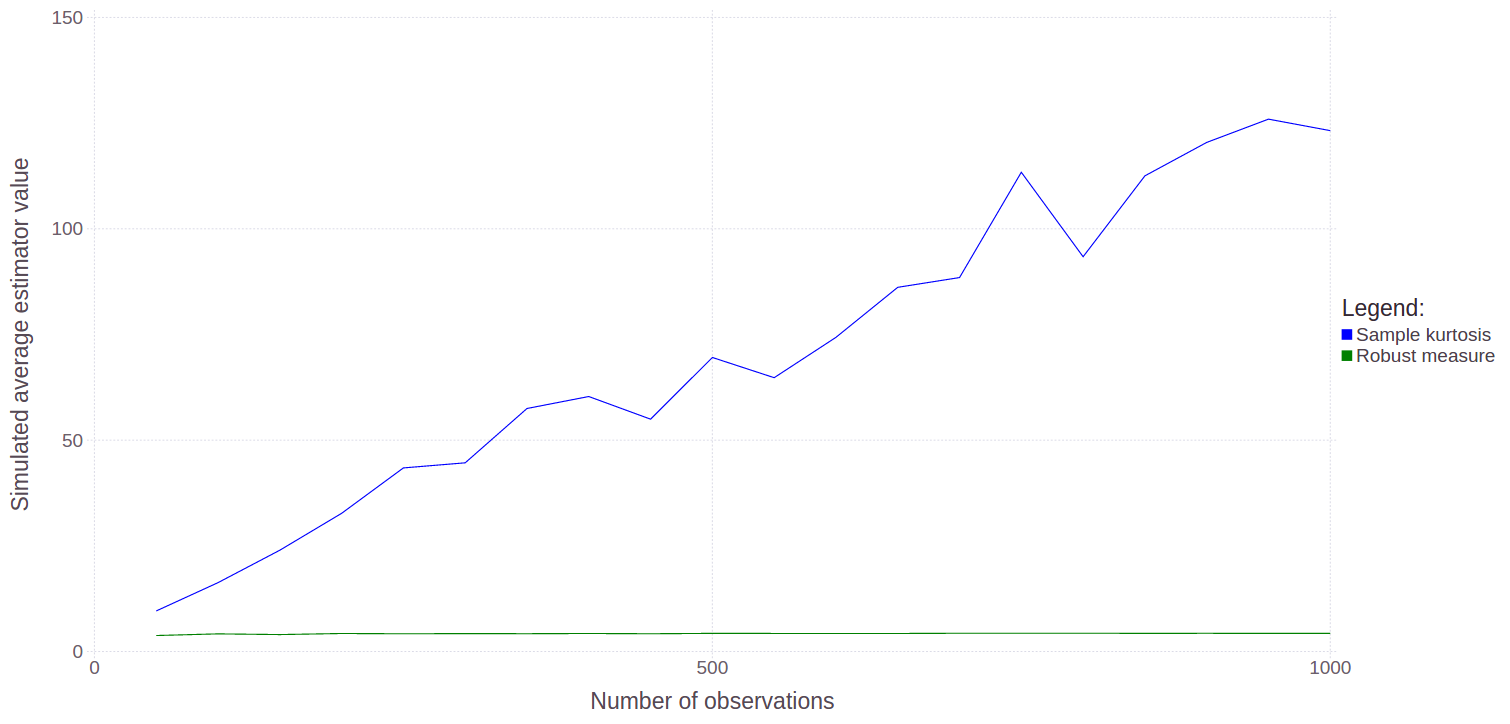
\includegraphics[height=5.0cm]{tDistSampleKurtosis}} \end{picture}
\end{center}
\vspace{0.75cm}
Sample kurtosis versus robust kurtosis for Student-t (2 DoF) DGP
\end{frame}




\section{Tail Fatness in Daily Financial Returns}


\begin{frame}
\frametitle{Tail Fatness in Daily Financial Returns}
\begin{center}
\begin{picture}(200,100) \put(-60,-30){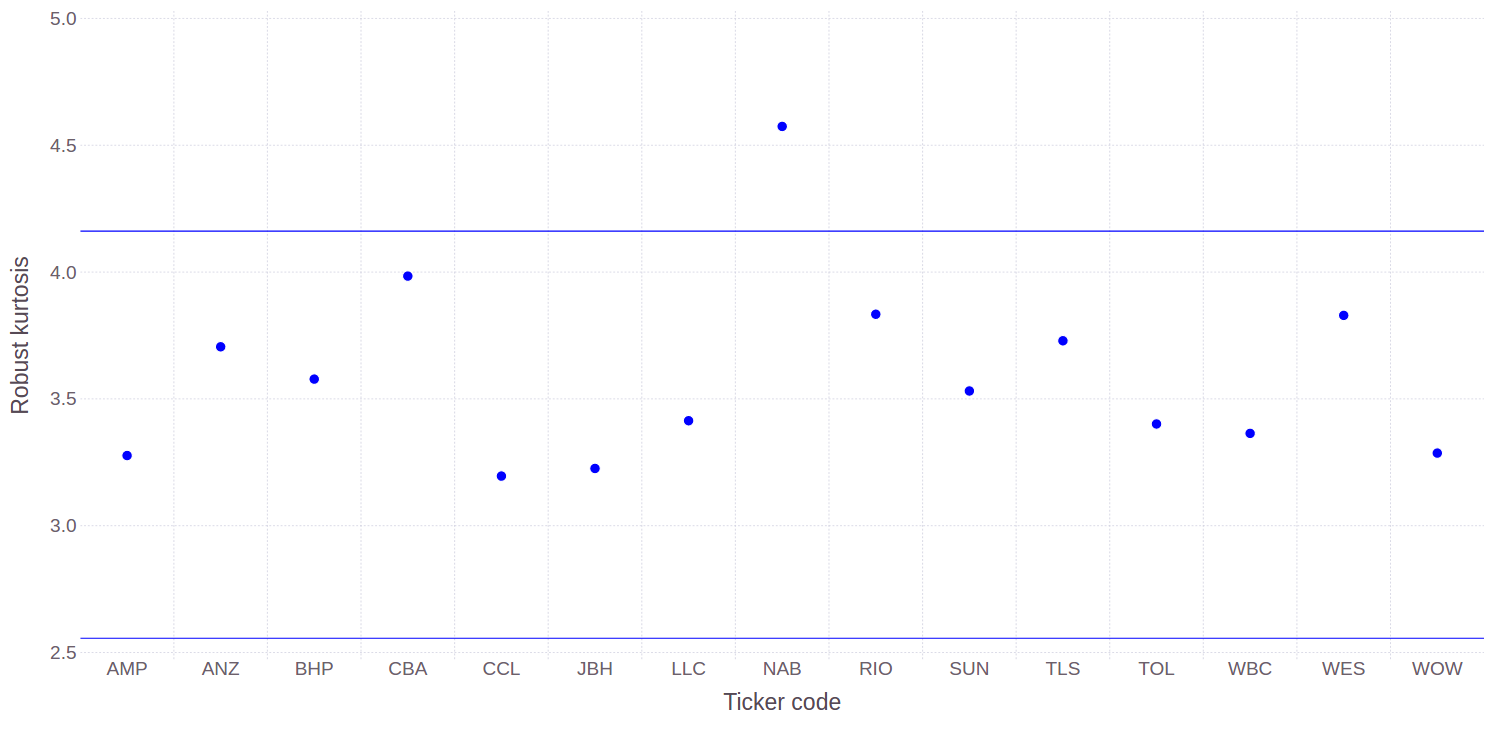
\includegraphics[height=5.0cm]{RobustKurtStocks}} \end{picture}
\end{center}
\vspace{0.75cm}
Robust kurtosis of daily financial returns for some popular stocks. Note, Normal and Student-t (2 DoF) lines included for reference. 
\end{frame}

\begin{frame}
\frametitle{A model for unconditional fat tails}
Unconditional fat tails can be generated by the model:
\begin{equation}
r_t \backsim \N(\m, \s_t^2) ,
\end{equation}
where $\s_t$ is typically stochastic, sometimes by conditioning on time $t-1$ (e.g. GARCH). 

\vspace{0.5cm}
The volatility clustering effect of GARCH results in short periods where, \emph{unconditionally}, we get many observations from the tails, e.g. late 2008 to early 2009.
\end{frame}

%
%\begin{frame}
%\frametitle{Tail Fatness in Daily Financial Returns}
%\begin{center}
%\begin{picture}(200,100) \put(-60,-30){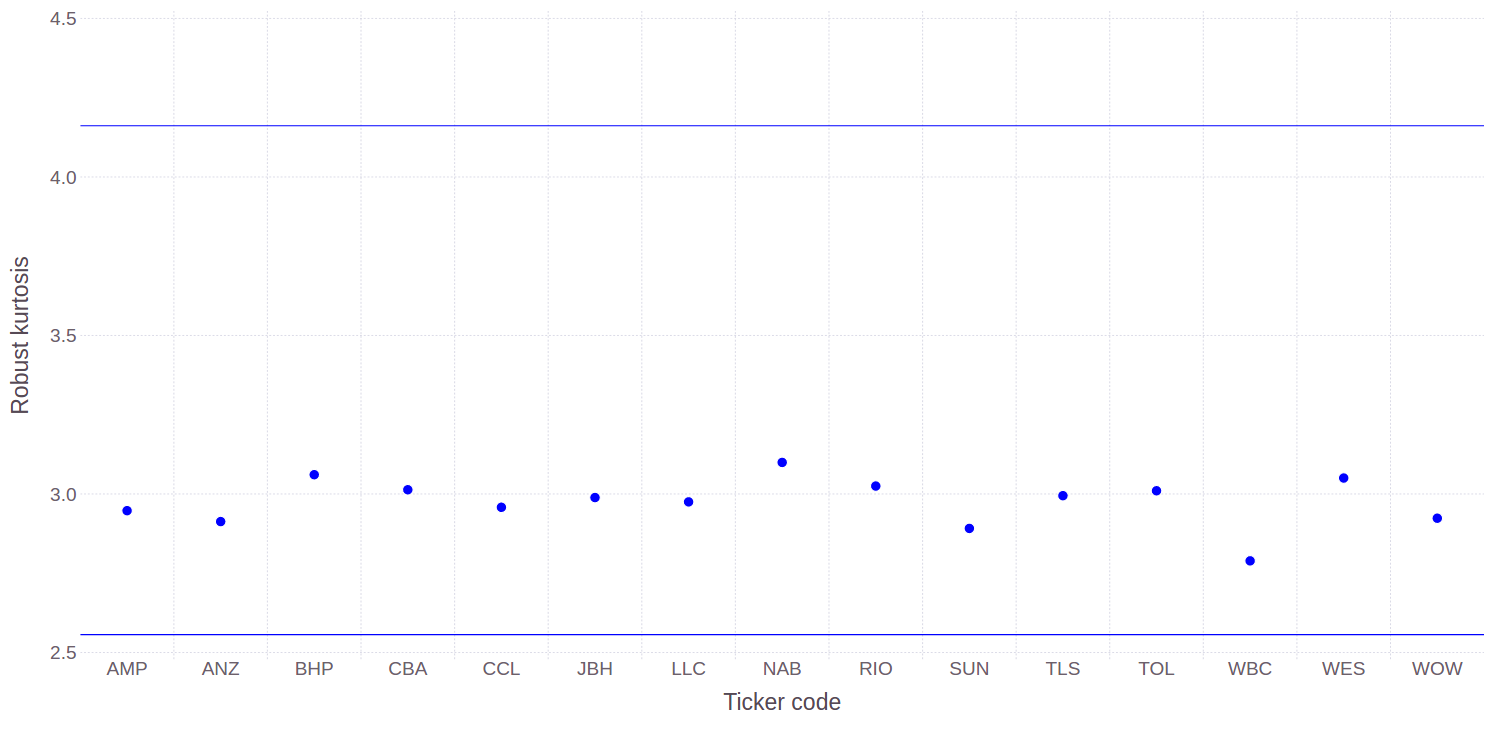
\includegraphics[height=5.0cm]{RobustKurtStocksStd}} \end{picture}
%\end{center}
%\vspace{0.75cm}
%Robust kurtosis of daily financial returns standardised by moving window* historical variance
%
%\scriptsize{*window length = 100}
%\end{frame}





\section{The Trimmed Mean for Daily Financial Returns}

%\begin{frame}
%\frametitle{The trimmed mean}
%Let $r_{[t]}, t = 1, ..., T$ denote the sorted version of $r_t, t = 1, ..., T$, (i.e. the \emph{order statistics}). Then the trimmed mean is defined:
%\begin{equation}
%m_\a = \frac{1}{(1 - \a)T} \sum_{t=\frac{a}{2}T}^{(1 - \frac{\a}{2})T} r_{[t]}
%\end{equation}
%for some $\a \in [0, 1]$.
%\vspace{0.5cm}
%
%Note:
%\begin{itemize}
%\item $\a = 0 \ra$ sample mean 
%\item $\a = 1 \ra$ sample median 
%\end{itemize}
%\end{frame}



\begin{frame}
\frametitle{Resampling financial returns}
\begin{itemize}
\item Start with a sequence of returns $r_t, t = 1, ..., T$
\item Centre the returns, i.e. $z_t = r_t - \bar{r}$
\item Sample (with replacement) blocks of observations from $z_t, t = 1, ..., T$. Denote a re-sampled observation $z_t^*$.
\item Under fairly general assumptions, $\E z_t^* = 0$, but $z_t$ will otherwise have ``similar'' statistical properties to $r_t$
\end{itemize}
\end{frame}



\begin{frame}
\frametitle{Kernel density estimates for trimmed and sample mean}
\begin{center}
\begin{picture}(200,100) \put(-60,-30){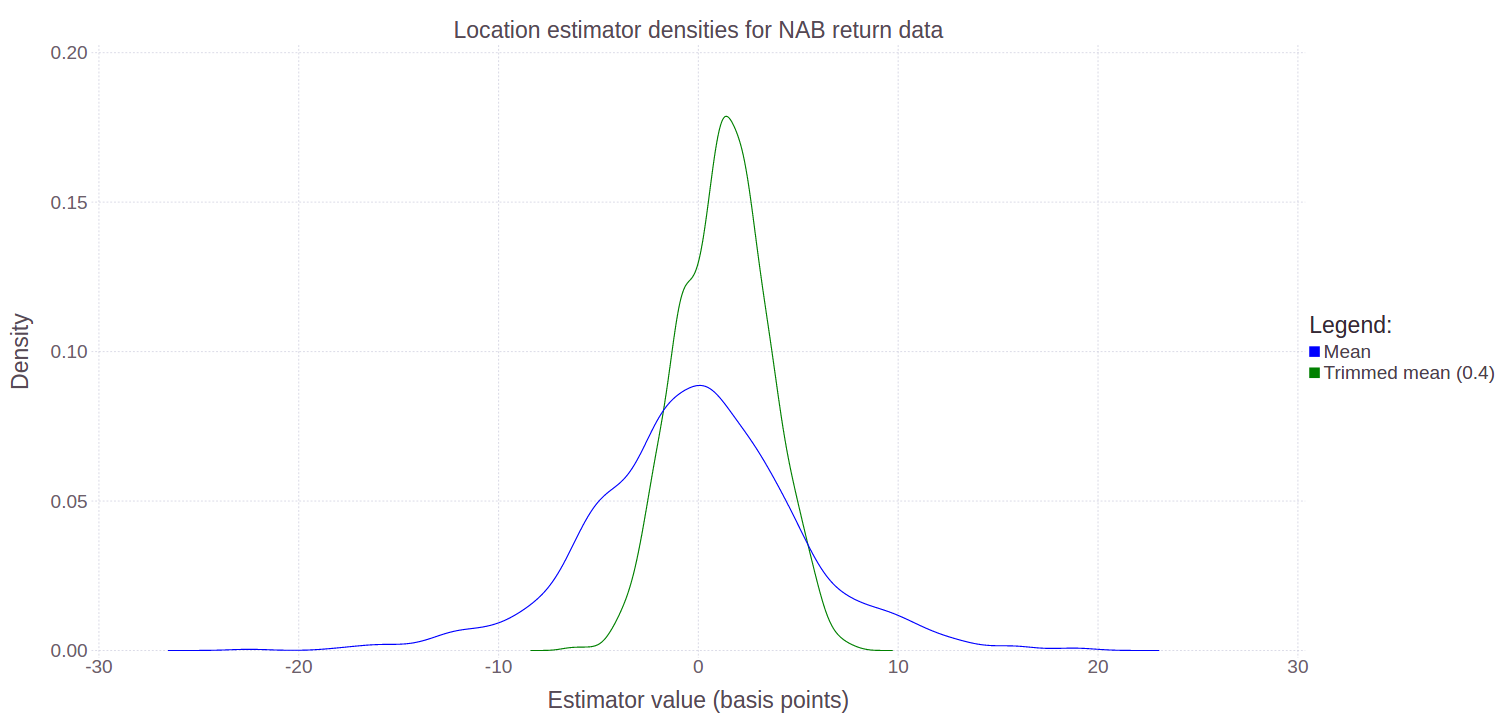
\includegraphics[height=5.0cm]{NABTrimMeanFullPeriod}} \end{picture}
\end{center}
\vspace{1cm}
Resampled NAB daily return data (2005 to 2015).
\end{frame}


\begin{frame}
\frametitle{Kernel density estimates for trimmed and sample mean}
\begin{center}
\begin{picture}(200,100) \put(-60,-30){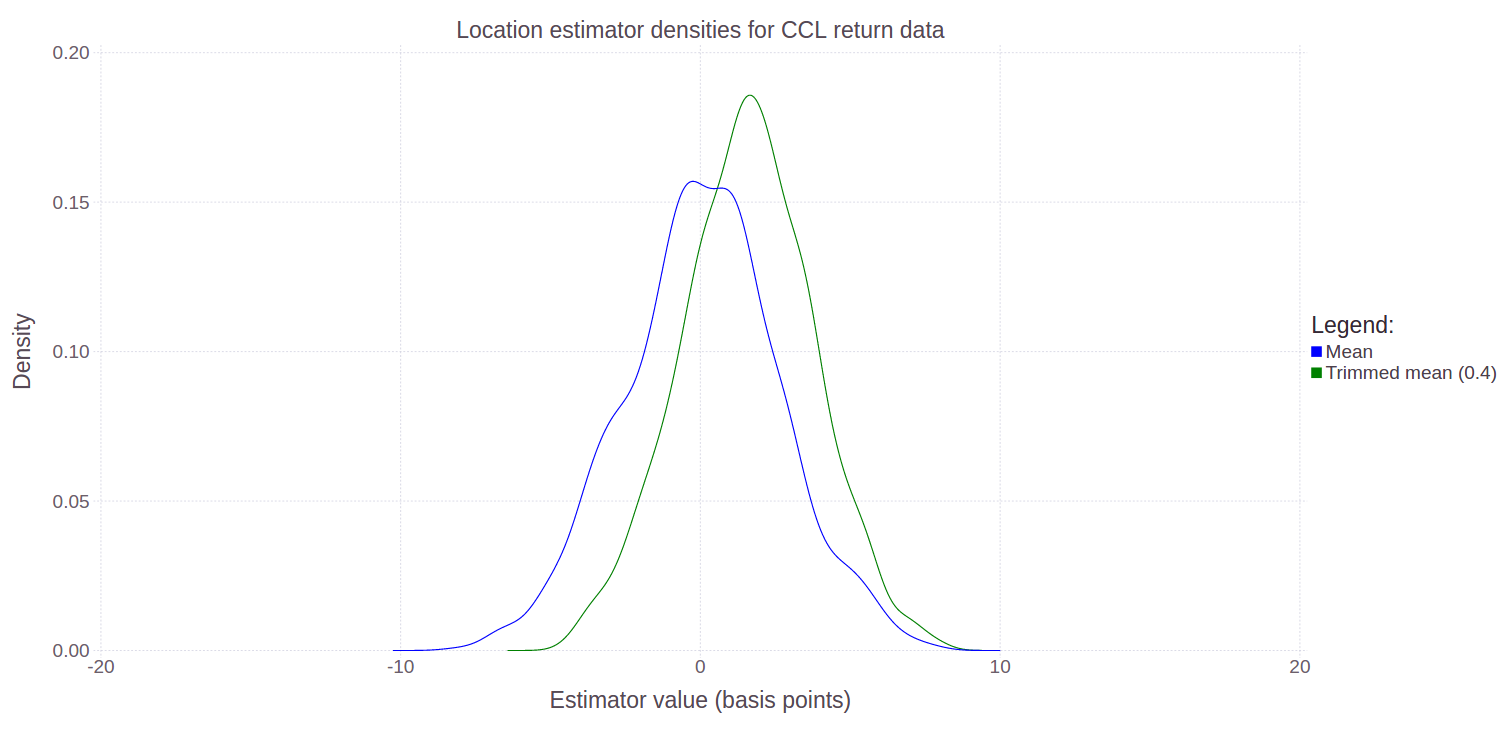
\includegraphics[height=5.0cm]{CCLTrimMeanFullPeriod}} \end{picture}
\end{center}
\vspace{1cm}
Resampled CCL daily return data (2005 to 2015).
\end{frame}



\begin{frame}
\frametitle{Kernel density estimates for trimmed and sample mean}
\begin{center}
\begin{picture}(200,100) \put(-60,-30){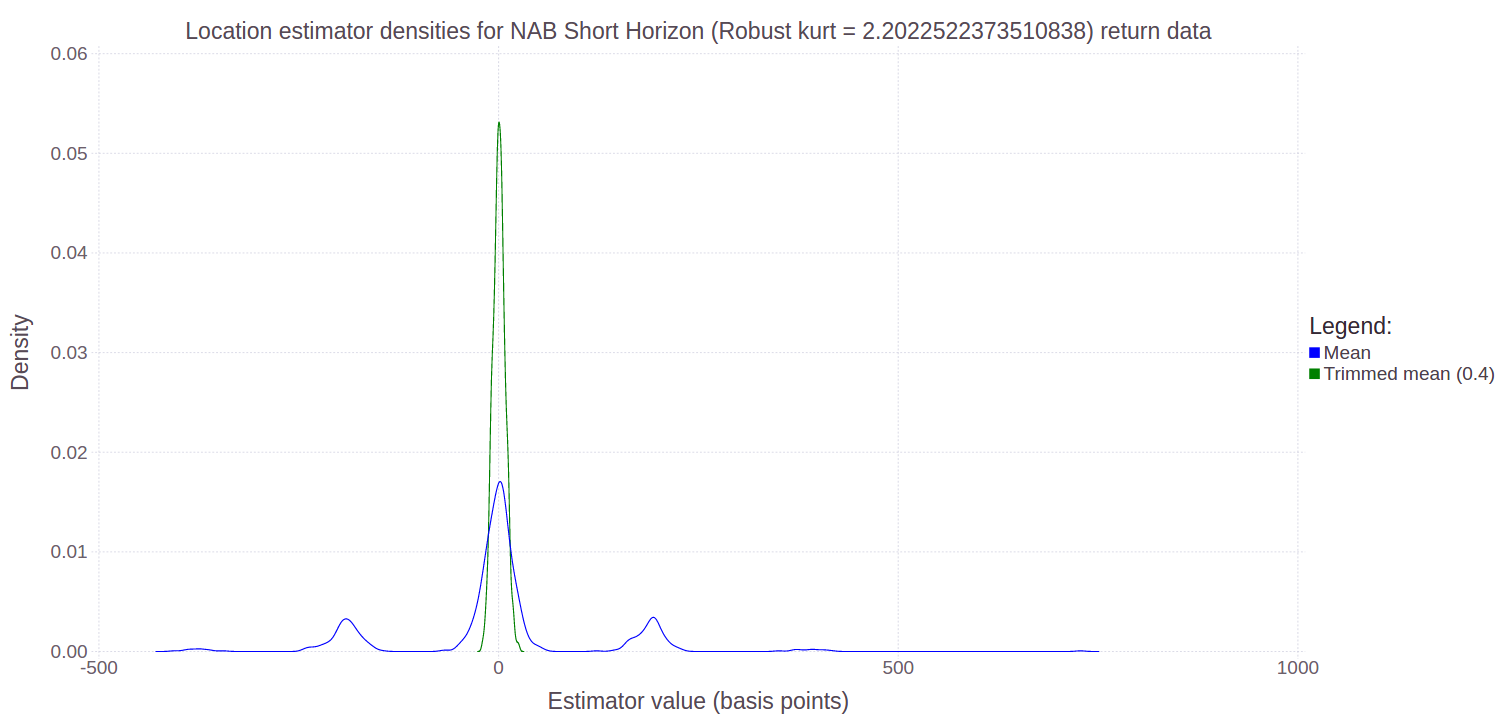
\includegraphics[height=5.0cm]{NABTrimMeanShortFat}} \end{picture}
\end{center}
\vspace{1cm}
Resampled NAB daily return data (100 sequential days with largest robust kurtosis).
\end{frame}



\begin{frame}
\frametitle{Kernel density estimates for trimmed and sample mean}
\begin{center}
\begin{picture}(200,100) \put(-60,-30){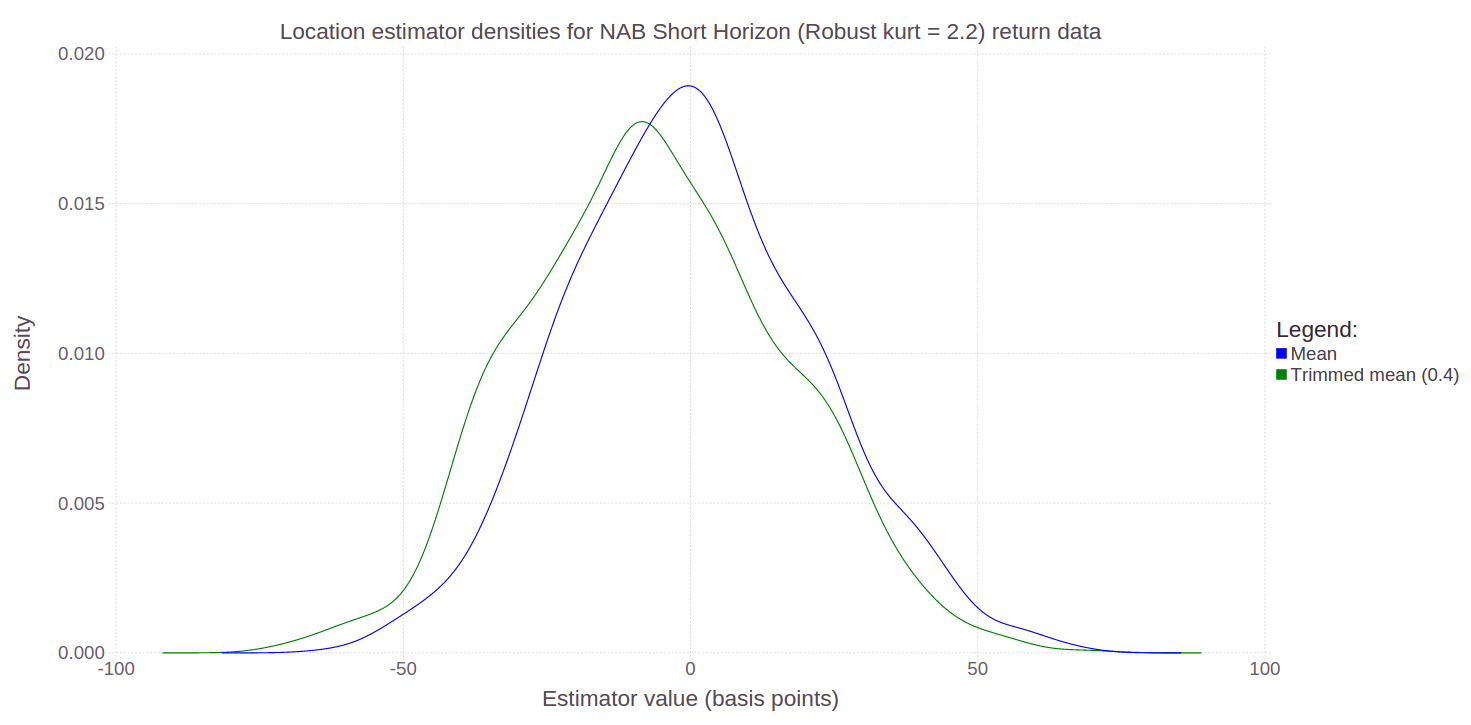
\includegraphics[height=5.0cm]{NABTrimMeanShortThin}} \end{picture}
\end{center}
\vspace{1cm}
Resampled NAB daily return data (100 sequential days with smallest robust kurtosis).
\end{frame}




\section{Robust Estimation of a Linear Model for Financial Returns}

\begin{frame}
\frametitle{A univariate linear model}
Assume daily returns are generated by the model:
\begin{equation}
r_t = \a + \b s_t + e_t ,
\end{equation}
where $s_t$ is a predictive signal.

\vspace{0.5cm}
\red{Note:} If the $R^2$ of this model is small, then $r_t$ and $e_t$ are likely to have similar statistical properties, such as heteroskedasticity.
\end{frame}


\begin{frame}
\frametitle{A broad class of estimators for a linear model}
Given observable data vectors $\bm{r}$ and $\bm{s}$, we have $\bm{e} = \bm{r} - \a - \b \bm{s}$.

A broad class of estimators for $\{\a, \b\}$ are the solution to the optimisation problem:
\begin{equation}
\min_{\a, \b} L(\bm{e}) ,
\end{equation}
for some loss function $L$.
\vspace{0.5cm}

\begin{itemize}
\item $L(\bm{e}) = \norm{\bm{e}}_2 \ra$ Least Squares (LS)
\item $L(\bm{e}) = \norm{\bm{e}}_1 \ra$ Least Absolute Deviations (LAD)
\end{itemize}
\blue{Question:} It is well know that LS loses its desirable properties in the presence of heteroskedasticity. So, given daily financial return data, should we prefer LS or LAD?
\end{frame}



\begin{frame}
\frametitle{Simulating data}
We want to simulate data using $r_t = \a + \b s_t + e_t$.
\begin{itemize}
\item Let $v_{t,\kappa}$ denote moving window historical variance on NAB returns, where $\kappa$ is window length
\item Use $e_t \backsim \N(0, v_{t,\kappa})$ to simulate residuals
\item Use $s_t \backsim \N(0, 1)$ to simulate signal
\item Set $\a = 0$, and choose $\b$ such that $R^2 = 0.05$
\item Simulate $r_t$
\end{itemize}
%\vspace{0.5cm}

\red{Note:}
\begin{itemize}
\item Both $r_t$ and $e_t$ will exhibit the same pattern of heteroskedasticity (similar to NAB)
\item $\kappa = 17$ results in robust kurtosis $\approx 4$ 
\end{itemize}
\end{frame}


\begin{frame}
\frametitle{Kernel density estimates for constant}
\begin{center}
\begin{picture}(200,100) \put(-60,-30){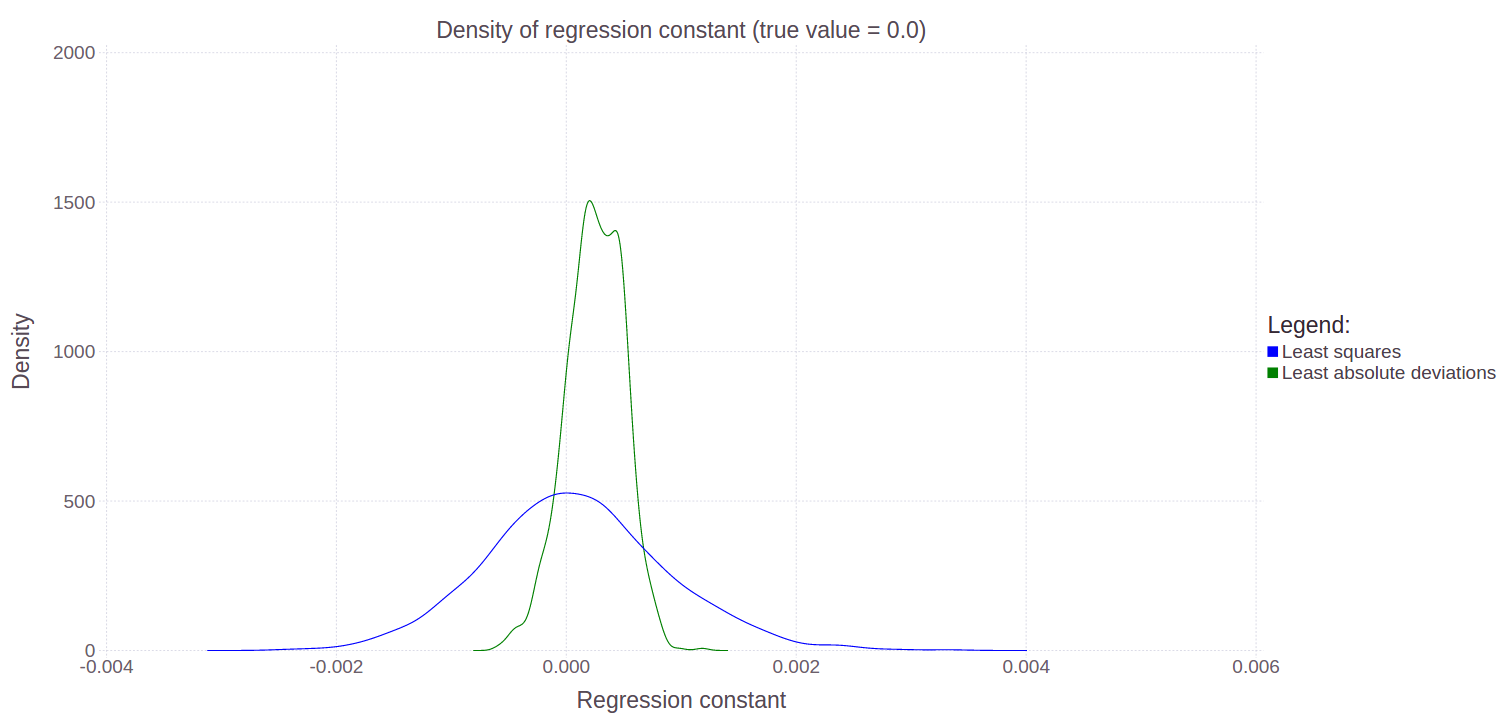
\includegraphics[height=5.0cm]{ConstantDensity}} \end{picture}
\end{center}
\end{frame}


\begin{frame}
\frametitle{Kernel density estimates for coefficient}
\begin{center}
\begin{picture}(200,100) \put(-60,-30){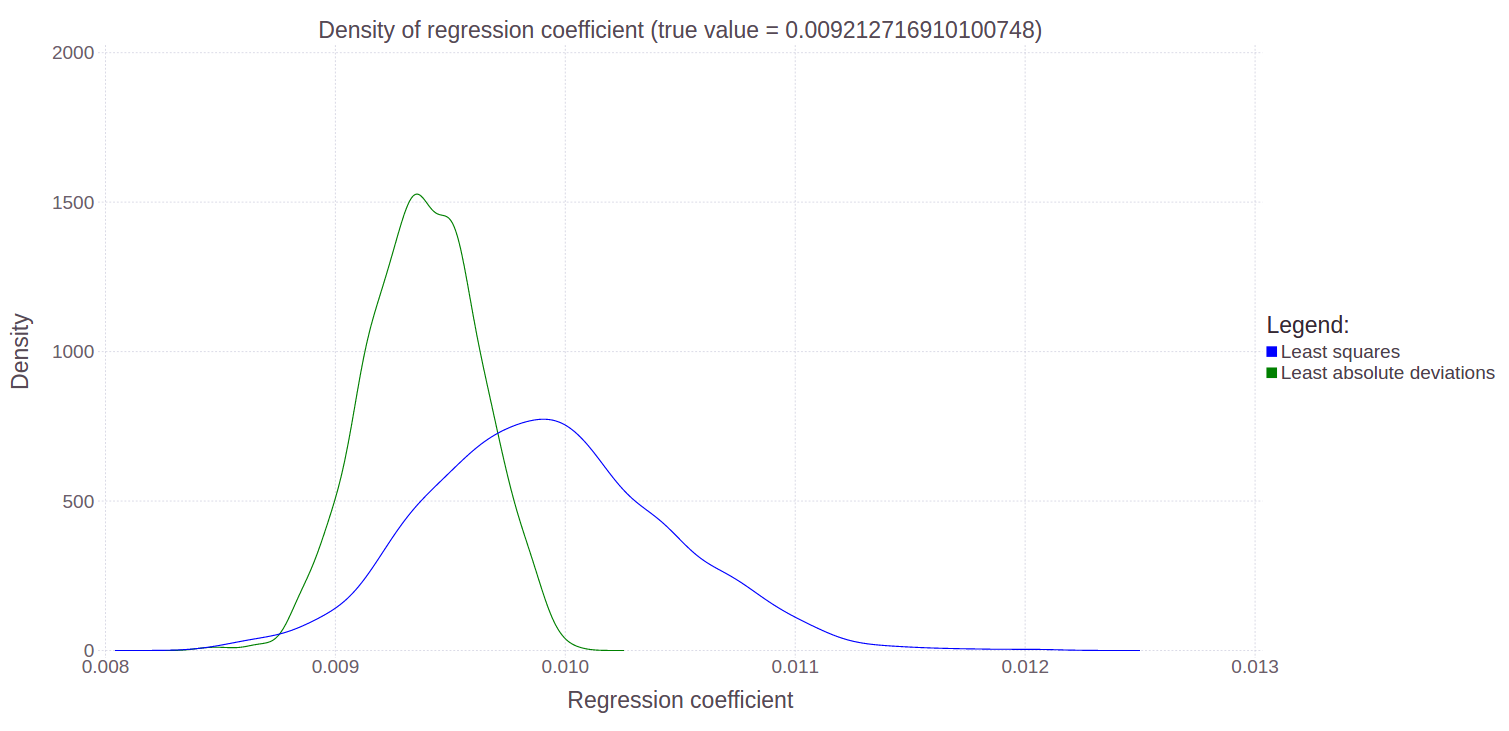
\includegraphics[height=5.0cm]{CoefDensity}} \end{picture}
\end{center}
\end{frame}



\begin{frame}
\frametitle{Implications for portfolio manager}
It immediately follows that LAD yields more accurate predictions. 

\blue{Question:} Does this translate to better returns?

\begin{itemize}
\item Simple economy with 20 assets plus zero-interest cash asset
\item Simulate all returns using method from previous slide
\item Estimate $\{\a, \b\}$ via LS and LAD using first half of sample
\item For second half, hold (equal-weighted) in period $t$ all assets with $\hat{r}_t = \hat{\a} + \hat{\b} s_t > 0$
\end{itemize}
\end{frame}



\begin{frame}
\frametitle{Kernel density estimates for terminal portfolio value}
\begin{center}
\begin{picture}(200,100) \put(-60,-30){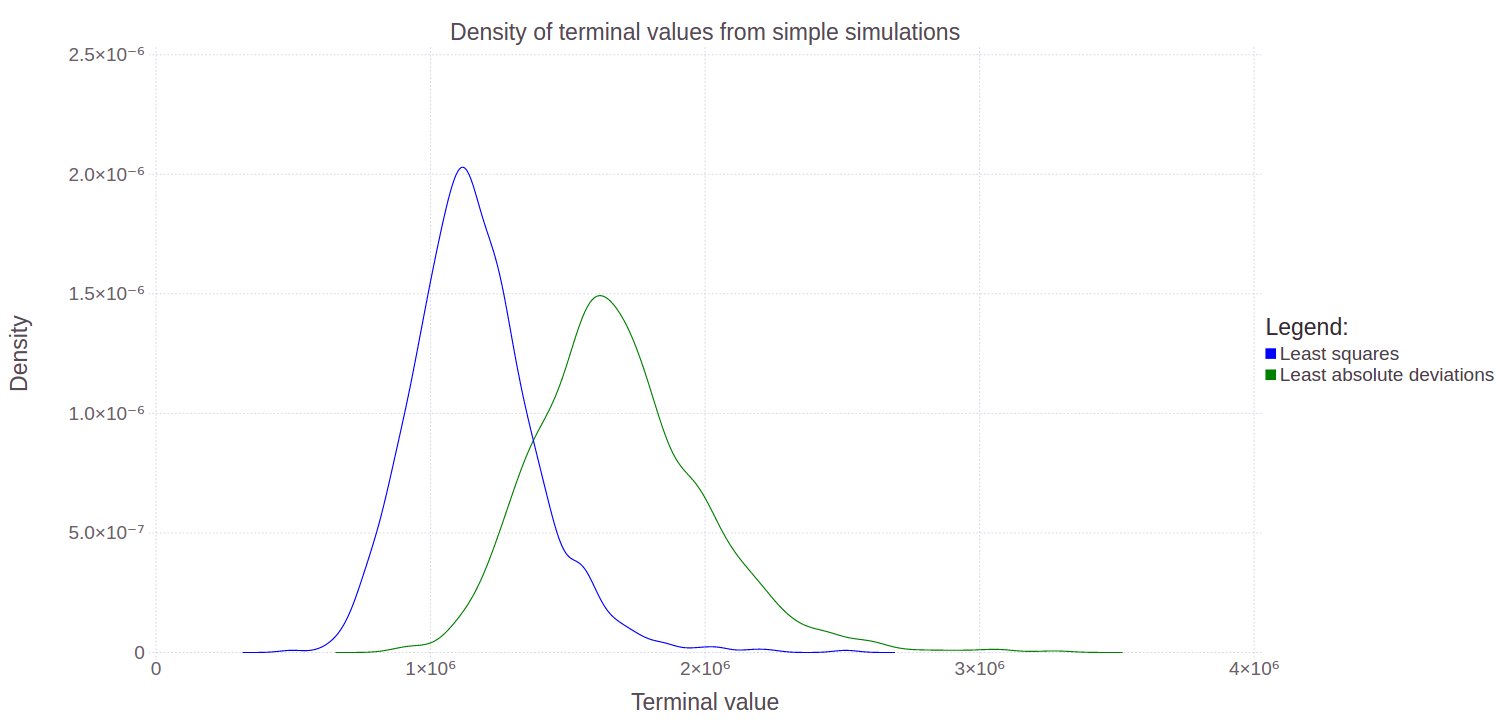
\includegraphics[height=5.0cm]{TradingSimTerminalVal}} \end{picture}
\end{center}
\vspace{1cm}

Portfolio terminal value for LS versus LAD estimation. Portfolio start value = 1 million.
\end{frame}




\section{What Can Go Wrong?}

\begin{frame}
\frametitle{Robust skew}
Let $Q_p$ denote the quantile corresponding to probability $p$. Then a robust measure of skewness is:
\begin{equation}
RobustSkewness = \frac{Q_{0.75} - Q_{0.5}}{Q_{0.75} - Q_{0.25}} - \frac{Q_{0.5} - Q_{0.25}}{Q_{0.75} - Q_{0.25}}
\end{equation}
\end{frame}



\begin{frame}
\frametitle{Robust skew}
\begin{center}
\begin{picture}(200,100) \put(-30,-30){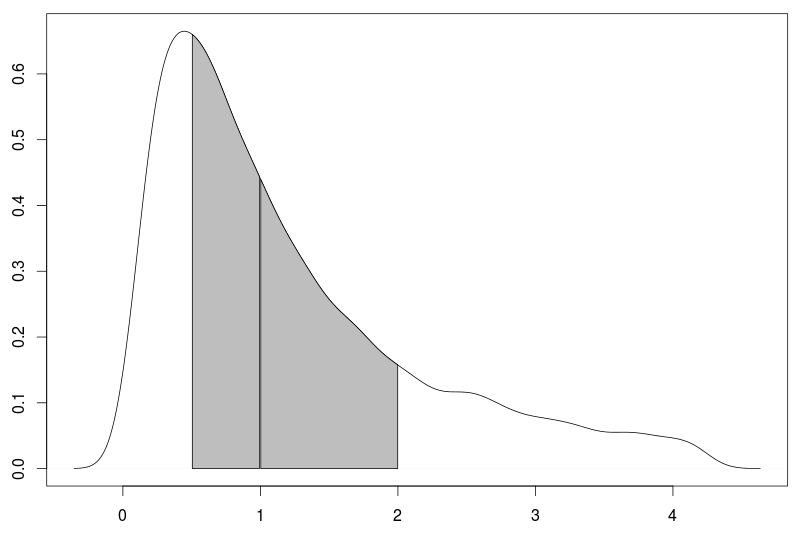
\includegraphics[height=5.0cm]{LognormalRobustSkewShaded}} \end{picture}
\end{center}
\vspace{0.5cm}

Kernel density of the Lognormal(0, 1) distribution with $0.25$, $0.5$, and $0.75$ quantiles marked
\end{frame}



\begin{frame}
\frametitle{Trim mean for Lognormal distribution}
\begin{center}
\begin{picture}(200,100) \put(-30,-30){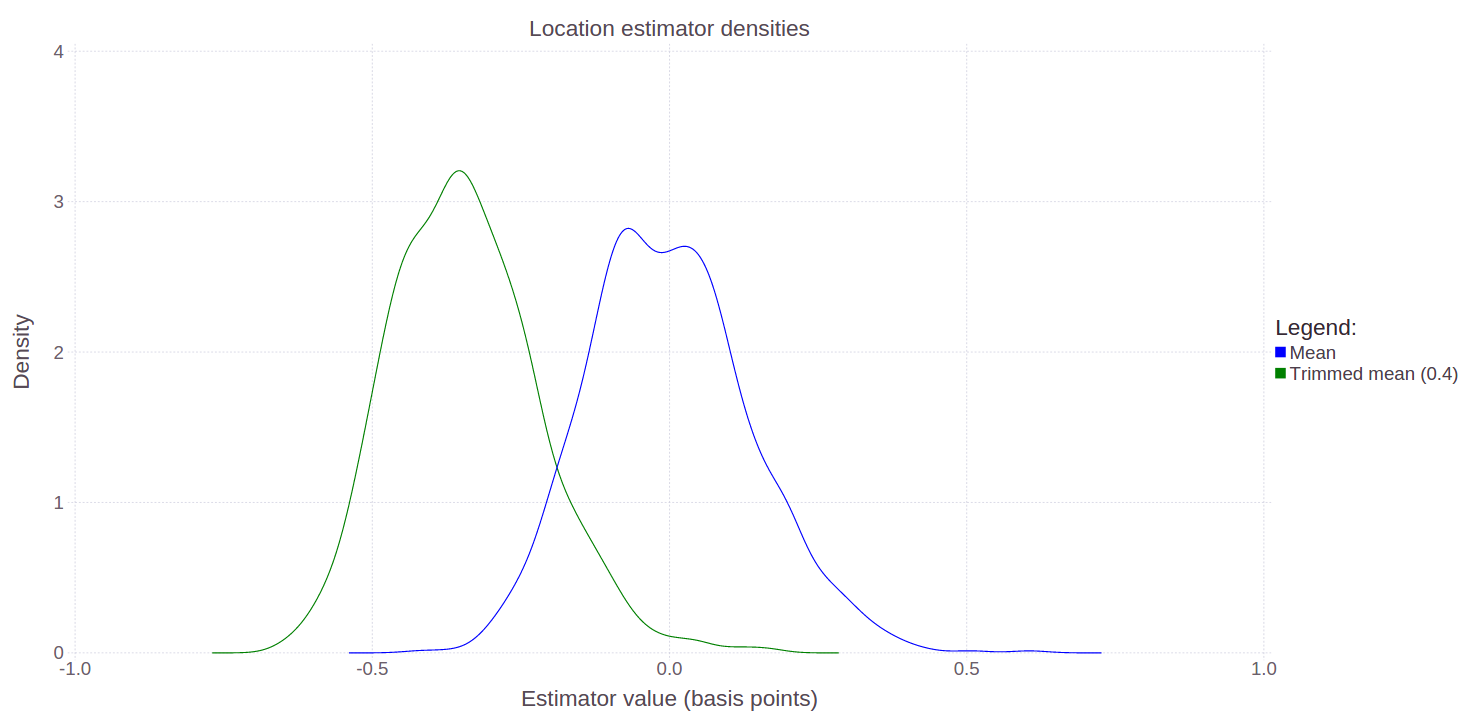
\includegraphics[height=5.0cm]{LognormalTrimMean}} \end{picture}
\end{center}
\begin{center}
\vspace{1.0cm}
True mean = 0
\end{center}
\end{frame}



\begin{frame}
\frametitle{Tail Fatness in Daily Financial Returns}
\begin{center}
\begin{picture}(200,100) \put(-60,-30){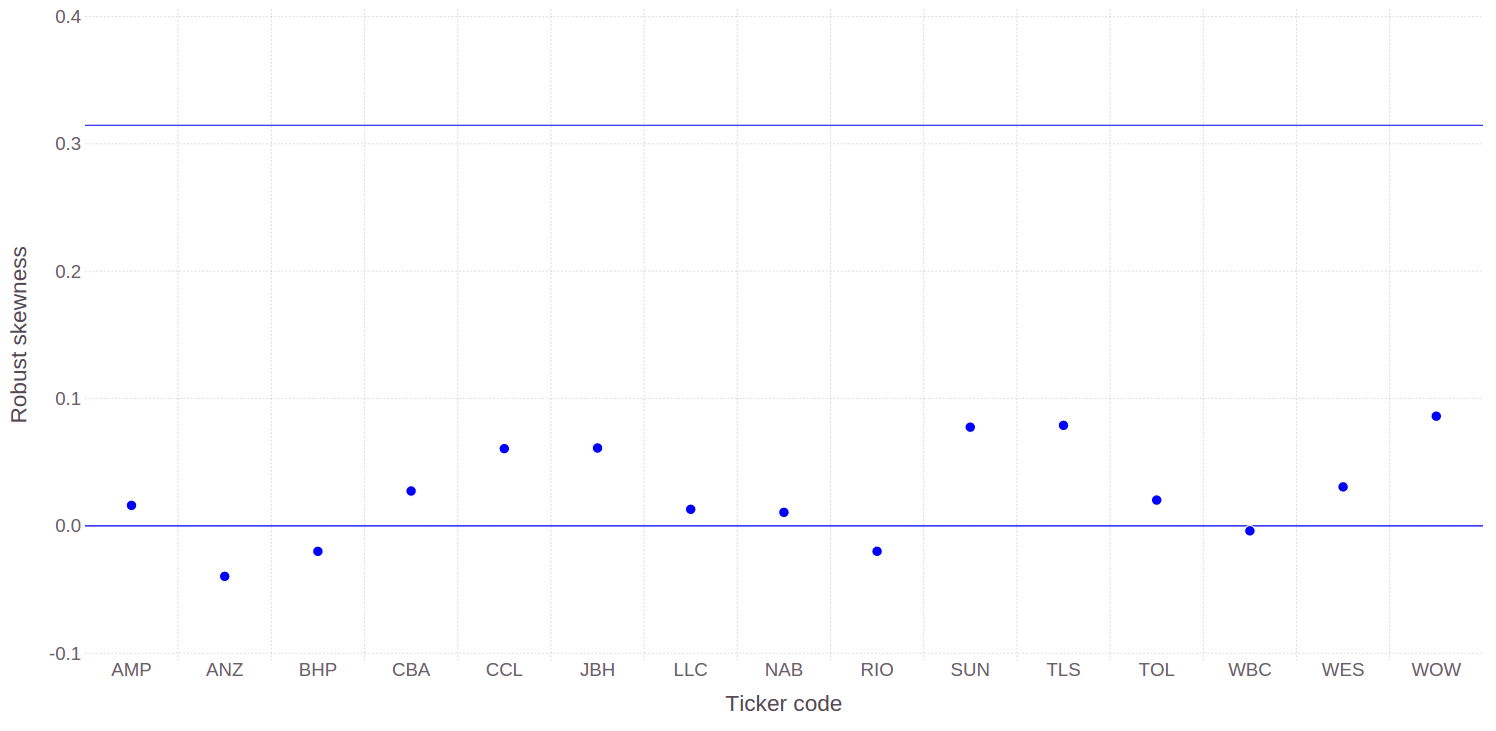
\includegraphics[height=5.0cm]{RobustSkewStocks}} \end{picture}
\end{center}
\vspace{0.75cm}
Robust skewness of daily financial returns for some popular stocks. Note, Symmetric and Lognormal(0, 1) lines included for reference. 
\end{frame}



\begin{frame}
\frametitle{Kernel density estimates for trimmed and sample mean}
\begin{center}
\begin{picture}(200,100) \put(-60,-30){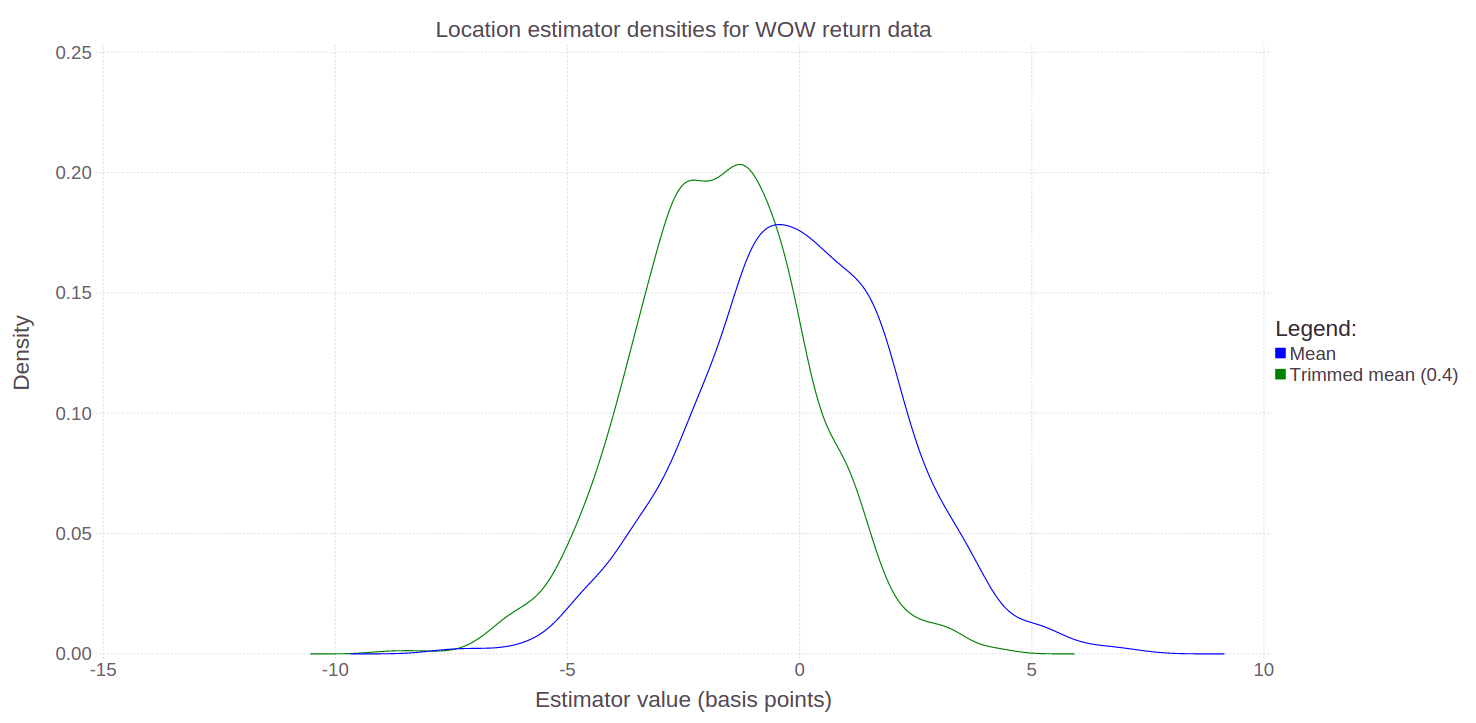
\includegraphics[height=5.0cm]{WOWTrimMeanFullPeriod}} \end{picture}
\end{center}
\vspace{1cm}
Resampled WOW daily return data (2005 to 2015).
\end{frame}



\begin{frame}
\frametitle{Kernel density estimates for trimmed and sample mean}
\begin{center}
\begin{picture}(200,100) \put(-60,-30){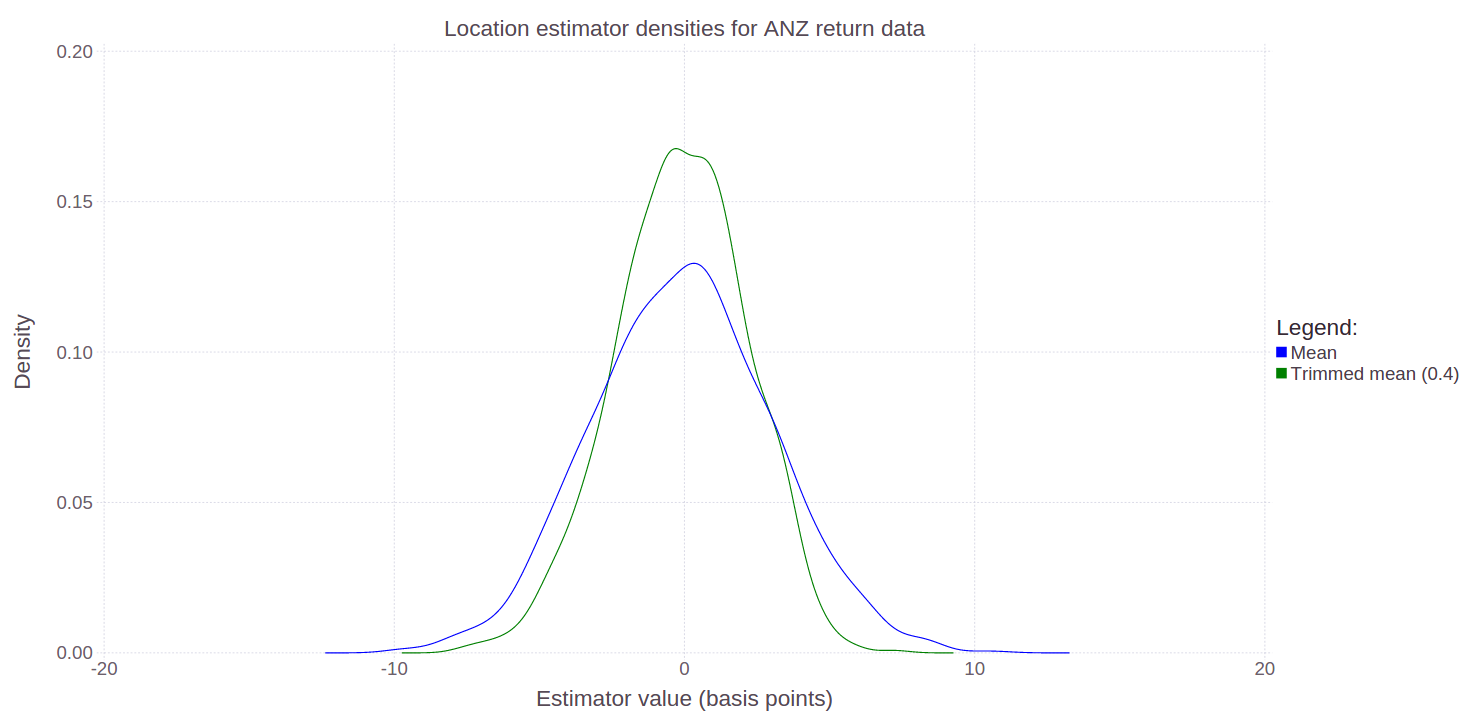
\includegraphics[height=5.0cm]{ANZTrimMeanFullPeriod}} \end{picture}
\end{center}
\vspace{1cm}
Resampled ANZ daily return data (2005 to 2015).
\end{frame}





\begin{frame}
\frametitle{TL;DR}
TL;DR: Any empiricist working with financial data subject to typical heteroskedasticity patterns should at least consider robust statistics.

\vspace{1cm}
All presentation materials and source code publicly available at:

\vspace{0.5cm}
\begin{center}
https://github.com/colintbowers/RobustStatsTutorial.jl
\end{center}
\end{frame}











%BELOW ARE SOME EXAMPLES ON THE INSERTGRAHPICS COMMAND
%\begin{frame}
%\frametitle{Noise}
%\includegraphics[height=4cm, clip=true, trim=0 0 0 225]{BidAskBounceExample}
%\includegraphics[totalheight=1\textheight, width=1\textwidth,viewport=0 0 580 480,clip]{BidAskBounceExample}
%\includegraphics[height=8cm,viewport=0 0 0 0,clip]{BidAskBounceExample}

%I LIKE THIS ONE IN PARTICULAR
%\begin{picture}(20, -20) \put(5, -5){\includegraphics[height=5cm]{NameOfFile}} \end{picture}

%BELOW IS AN EXAMPLE ON BUILDING YOUR OWN FRAME TO POSITION THE GRAPH
%\begin{frame}
%\framebox{
%	\begin{picture}(200,200)
%		\put(-20,-78){\includegraphics[height=13cm]{2006to2007DailyTradingVolume}}
%	\end{picture}
%		}
%\end{frame}


\end{document}
